\section{DRAMChannel Class Reference}
\label{classDRAMChannel}\index{DRAMChannel@{DRAMChannel}}
{\tt \#include $<$dram.h$>$}

Inheritance diagram for DRAMChannel:\nopagebreak
\begin{figure}[H]
\begin{center}
\leavevmode
\includegraphics[height=400pt]{classDRAMChannel__inherit__graph}
\end{center}
\end{figure}
Collaboration diagram for DRAMChannel:\nopagebreak
\begin{figure}[H]
\begin{center}
\leavevmode
\includegraphics[height=400pt]{classDRAMChannel__coll__graph}
\end{center}
\end{figure}
\subsection*{Public Member Functions}
\begin{CompactItemize}
\item 
{\bf DRAMChannel} ()
\item 
{\bf $\sim$DRAMChannel} ()
\item 
void {\bf process\_\-event} ({\bf IrisEvent} $\ast$e)
\item 
std::string {\bf toString} ()
\end{CompactItemize}
\subsection*{Public Attributes}
\begin{CompactItemize}
\item 
{\bf Component} $\ast$ {\bf mc}
\item 
{\bf Component} $\ast$ {\bf parent}
\item 
{\bf Component} $\ast$ {\bf child}
\item 
unsigned long long int {\bf dramBusyTime}
\item 
unsigned long long int {\bf dramBusyCycles}
\item 
unsigned long long int {\bf dramReadCycles}
\item 
unsigned long long int {\bf dramWriteCycles}
\item 
vector$<$ vector$<$ {\bf ullint} $>$ $>$ {\bf dramBankBusyTime}
\item 
vector$<$ vector$<$ {\bf ullint} $>$ $>$ {\bf dramBankBusyCycles}
\end{CompactItemize}


\subsection{Detailed Description}


Definition at line 35 of file dram.h.

\subsection{Constructor \& Destructor Documentation}
\index{DRAMChannel@{DRAMChannel}!DRAMChannel@{DRAMChannel}}
\index{DRAMChannel@{DRAMChannel}!DRAMChannel@{DRAMChannel}}
\subsubsection[{DRAMChannel}]{\setlength{\rightskip}{0pt plus 5cm}DRAMChannel::DRAMChannel ()}\label{classDRAMChannel_e4998aa7924b6f6a46966f62eed46f93}




Definition at line 113 of file dram.cc.\index{DRAMChannel@{DRAMChannel}!$\sim$DRAMChannel@{$\sim$DRAMChannel}}
\index{$\sim$DRAMChannel@{$\sim$DRAMChannel}!DRAMChannel@{DRAMChannel}}
\subsubsection[{$\sim$DRAMChannel}]{\setlength{\rightskip}{0pt plus 5cm}DRAMChannel::$\sim$DRAMChannel ()}\label{classDRAMChannel_bc6c60b5fb226ee24a986ddd5b1f1b80}




Definition at line 125 of file dram.cc.

\subsection{Member Function Documentation}
\index{DRAMChannel@{DRAMChannel}!process\_\-event@{process\_\-event}}
\index{process\_\-event@{process\_\-event}!DRAMChannel@{DRAMChannel}}
\subsubsection[{process\_\-event}]{\setlength{\rightskip}{0pt plus 5cm}void DRAMChannel::process\_\-event ({\bf IrisEvent} $\ast$ {\em e})}\label{classDRAMChannel_7a3494f58f927c1df099501d5b2daeba}




Definition at line 137 of file dram.cc.

References ACTIVATE, Request::address, ALL\_\-BANK\_\-REFRESH, Request::arrivalTime, Request::bankNo, child, DRAMCmdState::cmd, dramBankBusyCycles, dramBankBusyTime, dramBusyCycles, dramBusyTime, IrisEvent::event\_\-data, mc, NO\_\-OF\_\-BANKS, Simulator::Now(), PRECHARGE, DataBusHandler::process\_\-event(), Request::rankNo, READ, DRAMCmdState::req, Request::retireTime, Simulator::Schedule(), START\_\-READ, START\_\-WRITE, t\_\-CAS, t\_\-RCD, t\_\-RFC, t\_\-RP, t\_\-WR, IrisEvent::type, and WRITE.

Referenced by DataBusHandler::process\_\-event(), and CmdBusHandler::process\_\-event().

Here is the caller graph for this function:\nopagebreak
\begin{figure}[H]
\begin{center}
\leavevmode
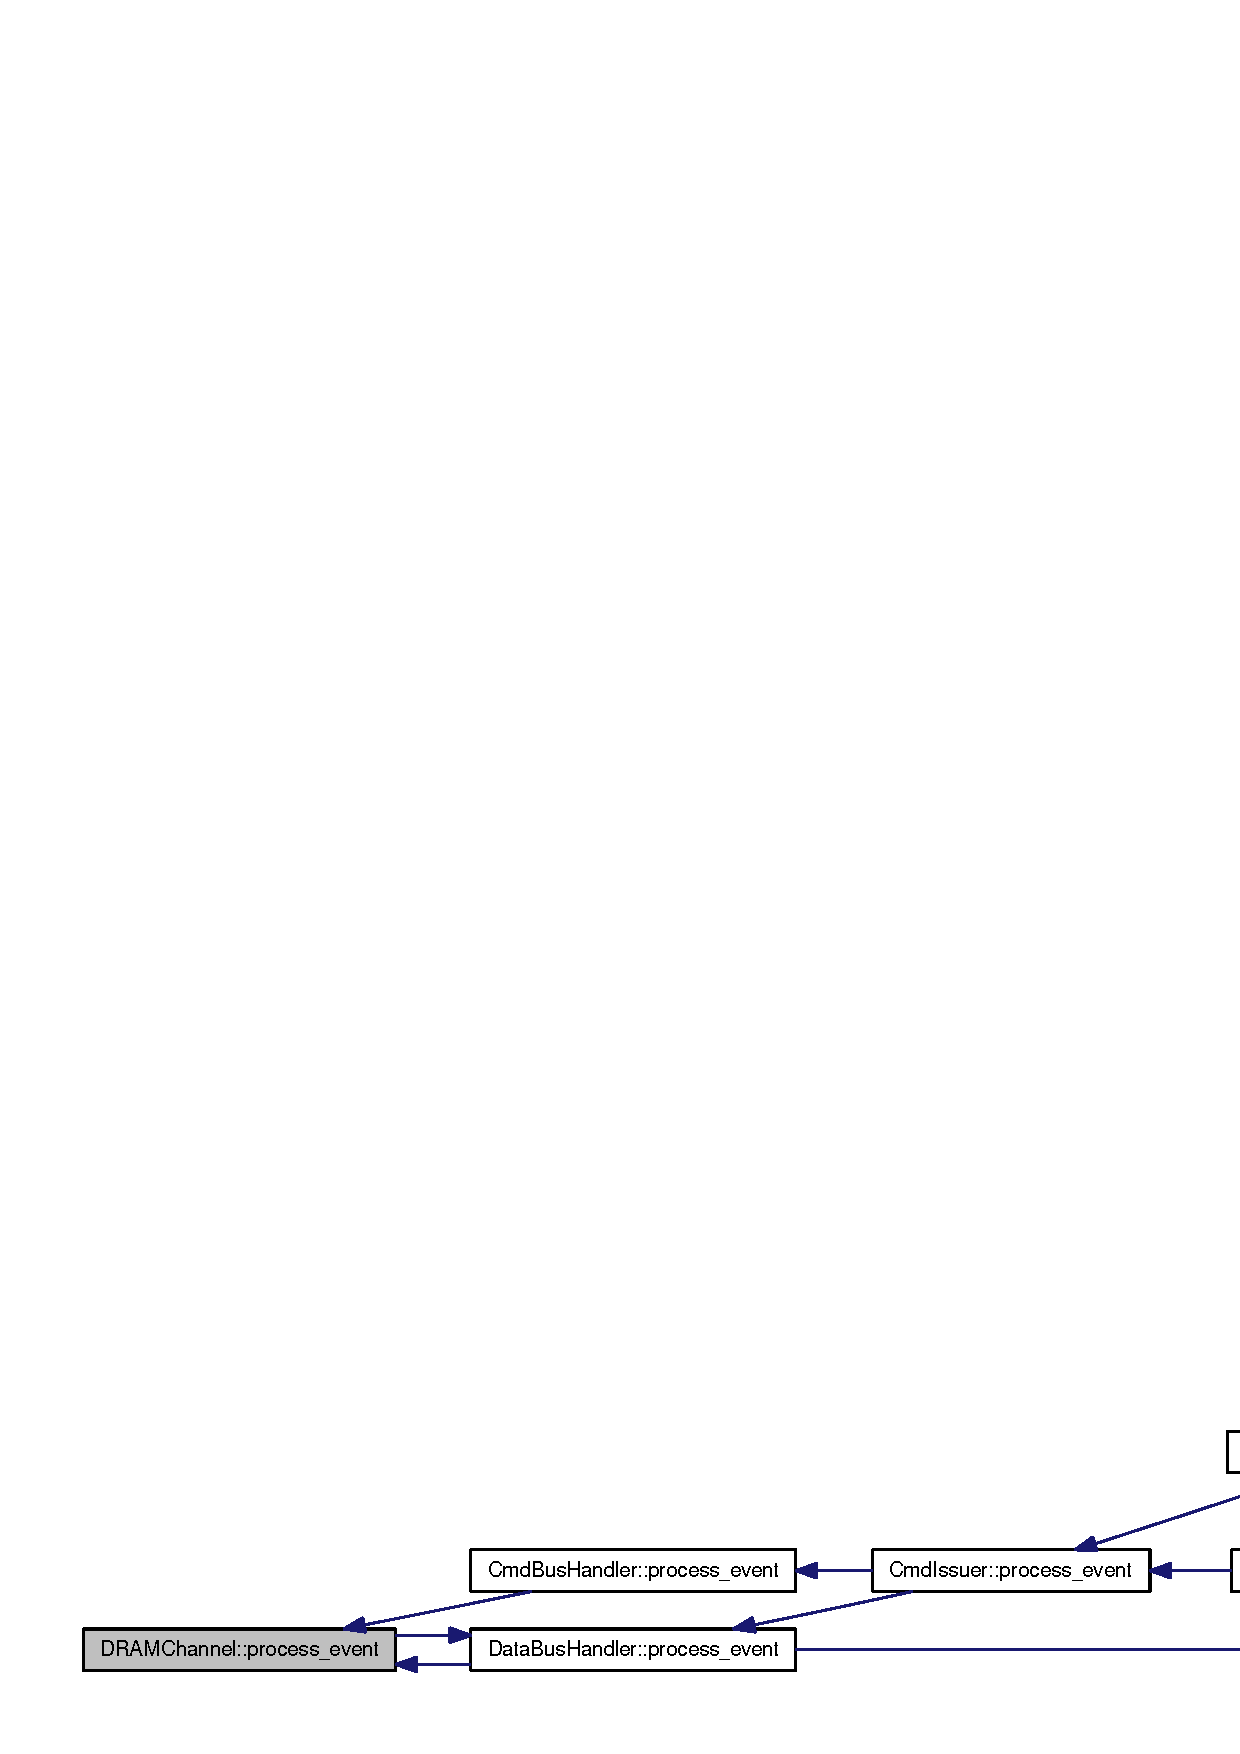
\includegraphics[width=420pt]{classDRAMChannel_7a3494f58f927c1df099501d5b2daeba_icgraph}
\end{center}
\end{figure}
\index{DRAMChannel@{DRAMChannel}!toString@{toString}}
\index{toString@{toString}!DRAMChannel@{DRAMChannel}}
\subsubsection[{toString}]{\setlength{\rightskip}{0pt plus 5cm}std::string DRAMChannel::toString ()}\label{classDRAMChannel_12db35357382fc91f7e382fe4a566e75}




\subsection{Member Data Documentation}
\index{DRAMChannel@{DRAMChannel}!child@{child}}
\index{child@{child}!DRAMChannel@{DRAMChannel}}
\subsubsection[{child}]{\setlength{\rightskip}{0pt plus 5cm}{\bf Component}$\ast$ {\bf DRAMChannel::child}}\label{classDRAMChannel_54be82cd0a97fc3dc05816d566d79be2}




Definition at line 42 of file dram.h.

Referenced by process\_\-event(), and DRAM::SetLinks().\index{DRAMChannel@{DRAMChannel}!dramBankBusyCycles@{dramBankBusyCycles}}
\index{dramBankBusyCycles@{dramBankBusyCycles}!DRAMChannel@{DRAMChannel}}
\subsubsection[{dramBankBusyCycles}]{\setlength{\rightskip}{0pt plus 5cm}vector$<$ vector$<${\bf ullint}$>$ $>$ {\bf DRAMChannel::dramBankBusyCycles}}\label{classDRAMChannel_222ef79694ef7c692f3fc52d30de2189}




Definition at line 51 of file dram.h.

Referenced by DRAM::DRAM(), and process\_\-event().\index{DRAMChannel@{DRAMChannel}!dramBankBusyTime@{dramBankBusyTime}}
\index{dramBankBusyTime@{dramBankBusyTime}!DRAMChannel@{DRAMChannel}}
\subsubsection[{dramBankBusyTime}]{\setlength{\rightskip}{0pt plus 5cm}vector$<$ vector$<${\bf ullint}$>$ $>$ {\bf DRAMChannel::dramBankBusyTime}}\label{classDRAMChannel_b9e0801464c6c4c3c6440493e4456486}




Definition at line 50 of file dram.h.

Referenced by DRAM::DRAM(), and process\_\-event().\index{DRAMChannel@{DRAMChannel}!dramBusyCycles@{dramBusyCycles}}
\index{dramBusyCycles@{dramBusyCycles}!DRAMChannel@{DRAMChannel}}
\subsubsection[{dramBusyCycles}]{\setlength{\rightskip}{0pt plus 5cm}unsigned long long int {\bf DRAMChannel::dramBusyCycles}}\label{classDRAMChannel_8d4533b55c2b44eb3f28ed99f3da1646}




Definition at line 47 of file dram.h.

Referenced by DRAM::DRAM(), and process\_\-event().\index{DRAMChannel@{DRAMChannel}!dramBusyTime@{dramBusyTime}}
\index{dramBusyTime@{dramBusyTime}!DRAMChannel@{DRAMChannel}}
\subsubsection[{dramBusyTime}]{\setlength{\rightskip}{0pt plus 5cm}unsigned long long int {\bf DRAMChannel::dramBusyTime}}\label{classDRAMChannel_c6893bec3a02f41d943302c633fe0775}




Definition at line 46 of file dram.h.

Referenced by DRAM::DRAM(), and process\_\-event().\index{DRAMChannel@{DRAMChannel}!dramReadCycles@{dramReadCycles}}
\index{dramReadCycles@{dramReadCycles}!DRAMChannel@{DRAMChannel}}
\subsubsection[{dramReadCycles}]{\setlength{\rightskip}{0pt plus 5cm}unsigned long long int {\bf DRAMChannel::dramReadCycles}}\label{classDRAMChannel_f61c93deaa124e78bc893c1be1cf639e}




Definition at line 48 of file dram.h.\index{DRAMChannel@{DRAMChannel}!dramWriteCycles@{dramWriteCycles}}
\index{dramWriteCycles@{dramWriteCycles}!DRAMChannel@{DRAMChannel}}
\subsubsection[{dramWriteCycles}]{\setlength{\rightskip}{0pt plus 5cm}unsigned long long int {\bf DRAMChannel::dramWriteCycles}}\label{classDRAMChannel_404772e399cc8358af961dd0343194d0}




Definition at line 49 of file dram.h.\index{DRAMChannel@{DRAMChannel}!mc@{mc}}
\index{mc@{mc}!DRAMChannel@{DRAMChannel}}
\subsubsection[{mc}]{\setlength{\rightskip}{0pt plus 5cm}{\bf Component}$\ast$ {\bf DRAMChannel::mc}}\label{classDRAMChannel_762802c40d545c267dd9109e1e013d69}




Definition at line 40 of file dram.h.

Referenced by process\_\-event(), and DRAM::SetLinks().\index{DRAMChannel@{DRAMChannel}!parent@{parent}}
\index{parent@{parent}!DRAMChannel@{DRAMChannel}}
\subsubsection[{parent}]{\setlength{\rightskip}{0pt plus 5cm}{\bf Component}$\ast$ {\bf DRAMChannel::parent}}\label{classDRAMChannel_ed6753935c84ed93dd15aea96a530aca}




Definition at line 41 of file dram.h.

Referenced by DRAM::SetLinks().

The documentation for this class was generated from the following files:\begin{CompactItemize}
\item 
{\bf dram.h}\item 
{\bf dram.cc}\end{CompactItemize}
